\documentclass{standalone}

\usepackage{tikz}
\usetikzlibrary{calc}

\begin{document}

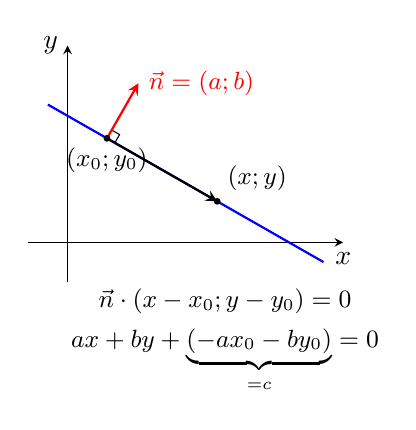
\begin{tikzpicture}[scale=1]

\draw[-stealth] (-0.5,0)--++(4,0) node[below] {$x$};
\draw[-stealth] (0,-0.5)--++(0,3) node[left] {$y$};
\draw[thick, blue] (-0.25,1.75)--(3.25,-0.25);

\draw (0.6,{-0.6*4/7+45/28})--++($0.015*(4,7)$)--++($0.015*(-7,4)$);
\draw[-stealth, thick, red] (0.5,{-0.5*4/7+45/28}) --++($0.1*(4,7)$) node[right] {\small{$\vec n = (a;b)$}};
\draw[fill=black] (0.5,{-0.5*4/7+45/28}) circle (1pt) node[below] {\small{$(x_0;y_0)$}};


\draw[-stealth, thick, black] (0.5,{-0.5*4/7+45/28}) --++($-0.2*(-7,4)$) node[above right] {\small{$(x;y)$}};
\draw[fill=black] (1.9,{-1.9*4/7+45/28}) circle (1pt);

\node at (2,-0.75) {\small{$\vec n \cdot (x-x_0;y-y_0)=0$}};
\node at (2,-1.5) {\small{$ax+by+\underbrace{(-ax_0-by_0)}_{=c}=0$}};

\end{tikzpicture}

\end{document}